\documentclass{report}

% Packages nécessaires
\usepackage[utf8]{inputenc}
\usepackage[T1]{fontenc}
\usepackage[french]{babel}
\usepackage{titlesec}
\usepackage{tocloft}
\usepackage{lipsum} % Package de remplissage de texte (à retirer dans le rapport final)
\usepackage{graphicx}
\usepackage{float} % pour l'option de placement [H]
\usepackage[colorlinks=true, linkcolor=blue, citecolor=green]{hyperref}
\usepackage{minted} % pour la coloration syntaxique
\usepackage{lipsum}
\usepackage{wrapfig}   % Pour l'enroulement du texte autour des images
\usepackage{array}

% Mathématiques
\usepackage{amsmath, amssymb}
\usepackage{amsthm}
\usepackage{mdframed}  % Package pour les cadres


\newmdtheoremenv{boxedproperty}{Propriété}[section]  % Crée un environnement encadré pour les propriétés


% Configuration de la page
\usepackage[a4paper, left=2.5cm, right=2.5cm, top=2.5cm, bottom=2.5cm]{geometry}

% Pour avoir le petit dessin de l'INSA en bas à droite de chaque page
\usepackage{background}
\backgroundsetup{
scale=1,
angle=0,
opacity=1,
color=black,
contents={\begin{tikzpicture}[remember picture,overlay]
\node at ([xshift=-0.8in,yshift=0.8in] current page.south east) % Adjust the position of the logo.
{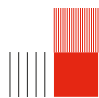
\includegraphics[scale=0.8]{images/pattern.png}}; % logo goes here
\end{tikzpicture}}
}


% Configuration des titres des sections et sous-sections
\titleformat{\chapter}[display]
  {\normalfont\Large\bfseries}{\chaptertitlename\thechapter}{14pt}{}
\titleformat{\section}
  {\normalfont\Large\bfseries}{\thesection}{1em}{}
\titleformat{\subsection}
  {\normalfont\large\bfseries}{\thesubsection}{1em}{}

% Configuration de la table des matières
\renewcommand{\cftchapfont}{\bfseries}
\renewcommand{\cftsecfont}{\normalfont}
\renewcommand{\cftsubsecfont}{\normalfont}
\renewcommand{\cftchappagefont}{\bfseries}
\renewcommand{\cftsecpagefont}{\normalfont}
\renewcommand{\cftsubsecpagefont}{\normalfont}
\setlength{\cftbeforetoctitleskip}{0pt}
\setlength{\cftaftertoctitleskip}{10pt}
\renewcommand{\contentsname}{Table des matières}



\begin{document}


% Page de titre
\begin{titlepage}
    \centering

    % Minipages pour les logos
    \noindent % Assure qu'il n'y a pas d'indentation au début de la ligne
    \begin{minipage}{0.5\textwidth}
        
\includegraphics[width=0.5\linewidth]{images/logo_INSA.png} % Ajustez le chemin et la taille
    \end{minipage}%
    \hfill % Assure que les deux minipages seront poussés à l'extrême gauche et droite
    \begin{minipage}{0.5\textwidth}
        \flushright % Alignement à droite dans la minipage
        
\includegraphics[width=0.5\linewidth]{images/blanc.jpg} % Ajustez le chemin et la taille
    \end{minipage}


    \vspace*{2cm} % Espace vertical de 2 cm
    {\Huge\bfseries Optimisation et parallelisation OpenMP d'addition et produit
de deux matrices denses \par}
    \vspace{1cm}
    {\huge Rapport de Burreau d'étude\par}
    \vspace{2cm}
    {\Large \textbf{Luc-Christelle Nguyen et Alicia Perrin} \par}
    \vspace{2cm}
    
    {\Large \textbf{Institut National des Sciences Appliquées de Toulouse} \par}
    \vspace{1cm}
    {\large \today \par}
\end{titlepage}

% Résumé concis, souvent utilisé pour donner un aperçu rapide du contenu d'une recherche ou d'un article académique.
\begin{abstract}
  Dans ce rapport, nous allons tester plusieurs méthodes différentes afin d'optimiser des calculs matriciels (somme, produit scalaire, produit matricielle). A COMPLETER
\end{abstract}

% Table des matières
\tableofcontents

\newpage


\chapter{Modifier l'accès à la mémoire pour additionner deux matrices}

\begin{figure}[H]
    \centering
    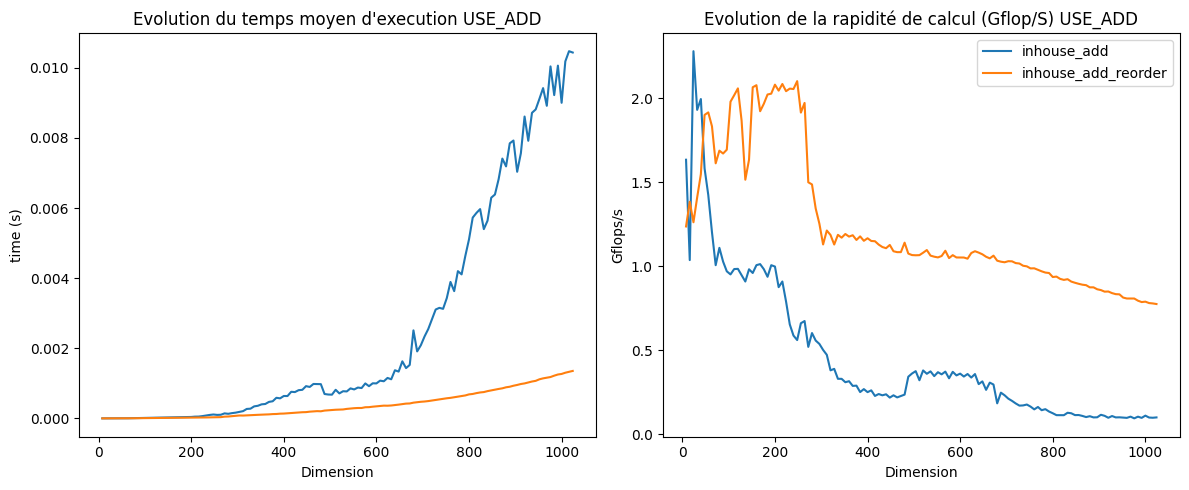
\includegraphics[width=0.7\linewidth]{images/fig3.png}
    \caption{Différences de performances en fonction de l'ordre d'accès à la mémoire}
    \label{fig:3}
\end{figure}

Modification de l'ordre d'accès à la mémoire : On lit d'abord les lignes pour une meilleure utilisation du cache. L'efficassité est doublée en moyenne.



\chapter{Compilation reliant les librairies OpenMP et BLAS}

ECRIRE EN FRANCAIS CE QUE FONT LES BLAS

\begin{figure}[H]
    \centering
    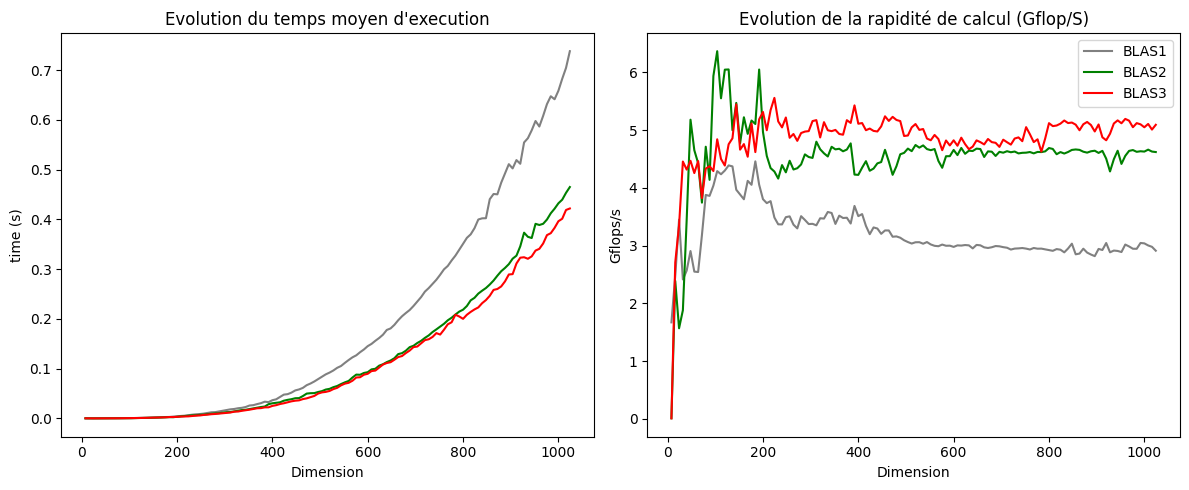
\includegraphics[width=0.7\linewidth]{images/fig1.png}
    \caption{Performances BLAS 1, 2, 3 sans optimisation Openblas}
    \label{fig:1}
\end{figure}

\begin{figure}[H]
    \centering
    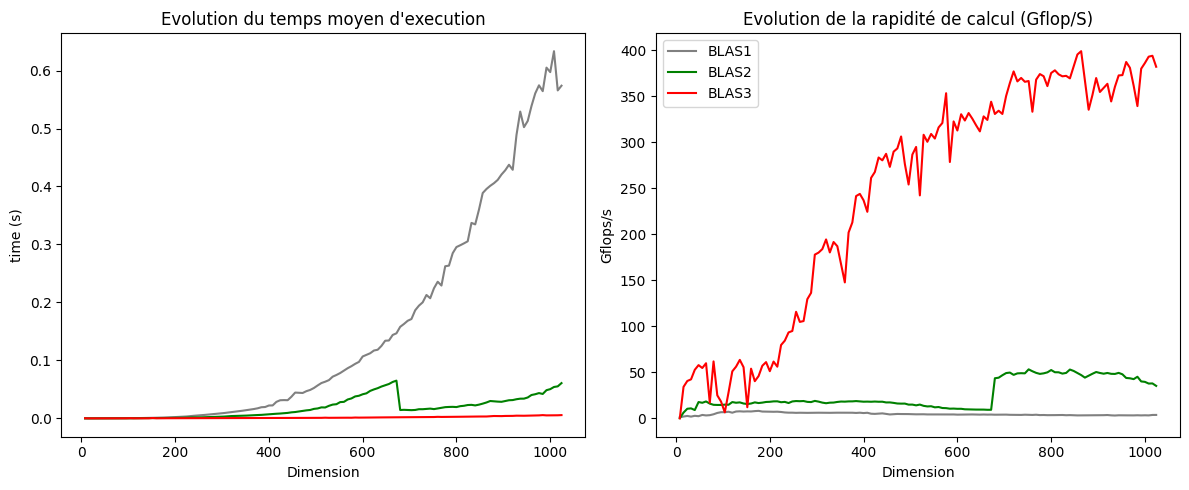
\includegraphics[width=0.7\linewidth]{images/fig2.png}
    \caption{Performances BLAS 1, 2, 3 avec optimisation Openblas}
    \label{fig:2}
\end{figure}

On peut voir une nete amélioration des performances lorsque on utilise la librairie openblas qui ... mettre ce qu'elle fait ... .
Pour BLAS3 5Gflops -> 400Gflops.

\chapter{Parallelisation OpenMP CHANGER}

\begin{figure}[H]
    \centering
    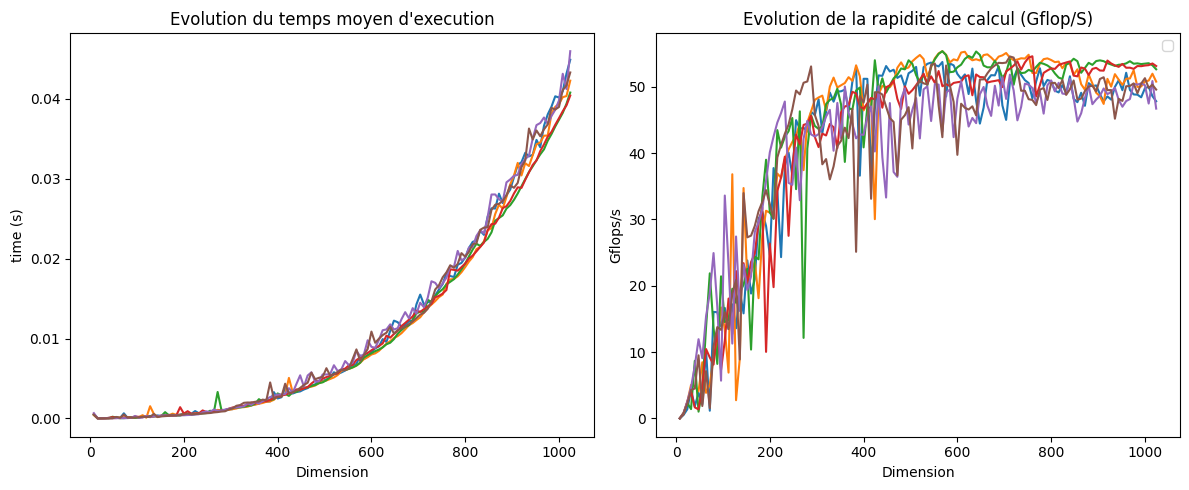
\includegraphics[width=0.7\linewidth]{images/fig4.png}
    \caption{Trouver titre}
    \label{fig:4}
\end{figure}

\begin{figure}[H]
    \centering
    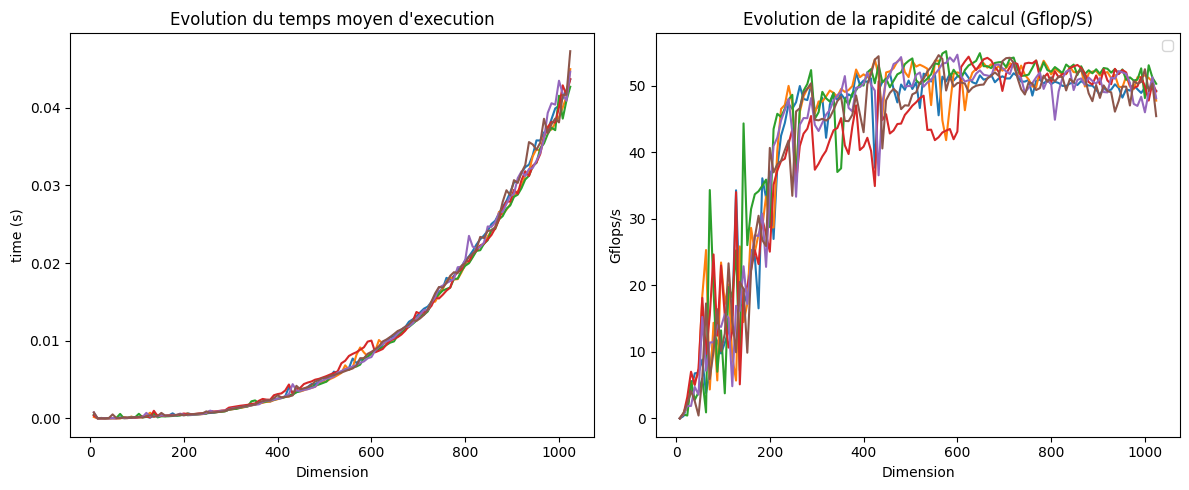
\includegraphics[width=0.7\linewidth]{images/fig5.png}
    \caption{Trouver titre}
    \label{fig:5}
\end{figure}

Comparer les option de parallelisation Static et Dynamique avec des nombres de Thread différents. On peut remarquer que cchanger ses options n'a pas une réelle influence.

\chapter{Nombre de threads utilisé pour BLAS3}
\begin{figure}[H]
    \centering
    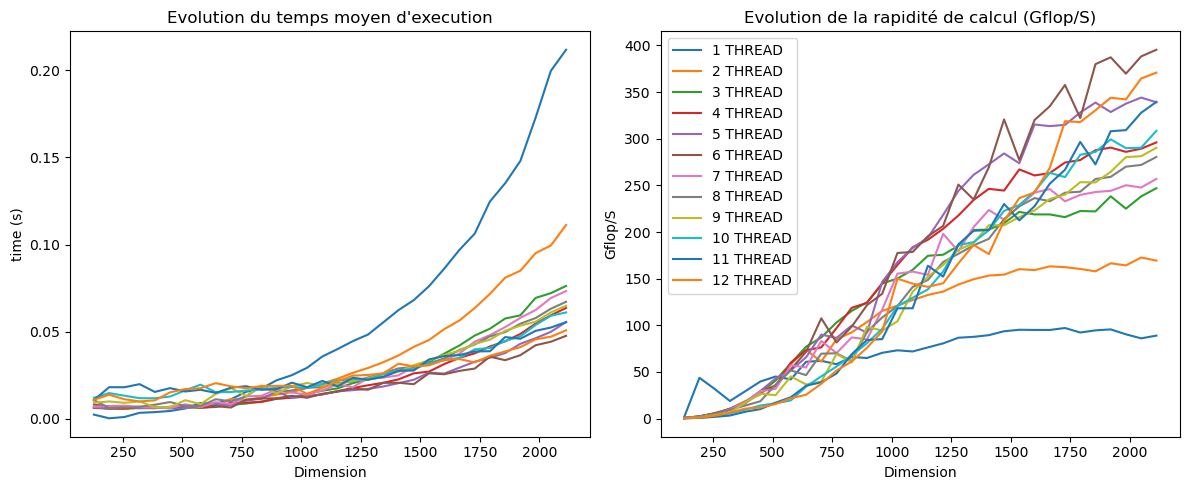
\includegraphics[width=0.7\linewidth]{images/fig6.png}
    \caption{Trouver titre}
    \label{fig:6}
\end{figure}

\begin{figure}[H]
    \centering
    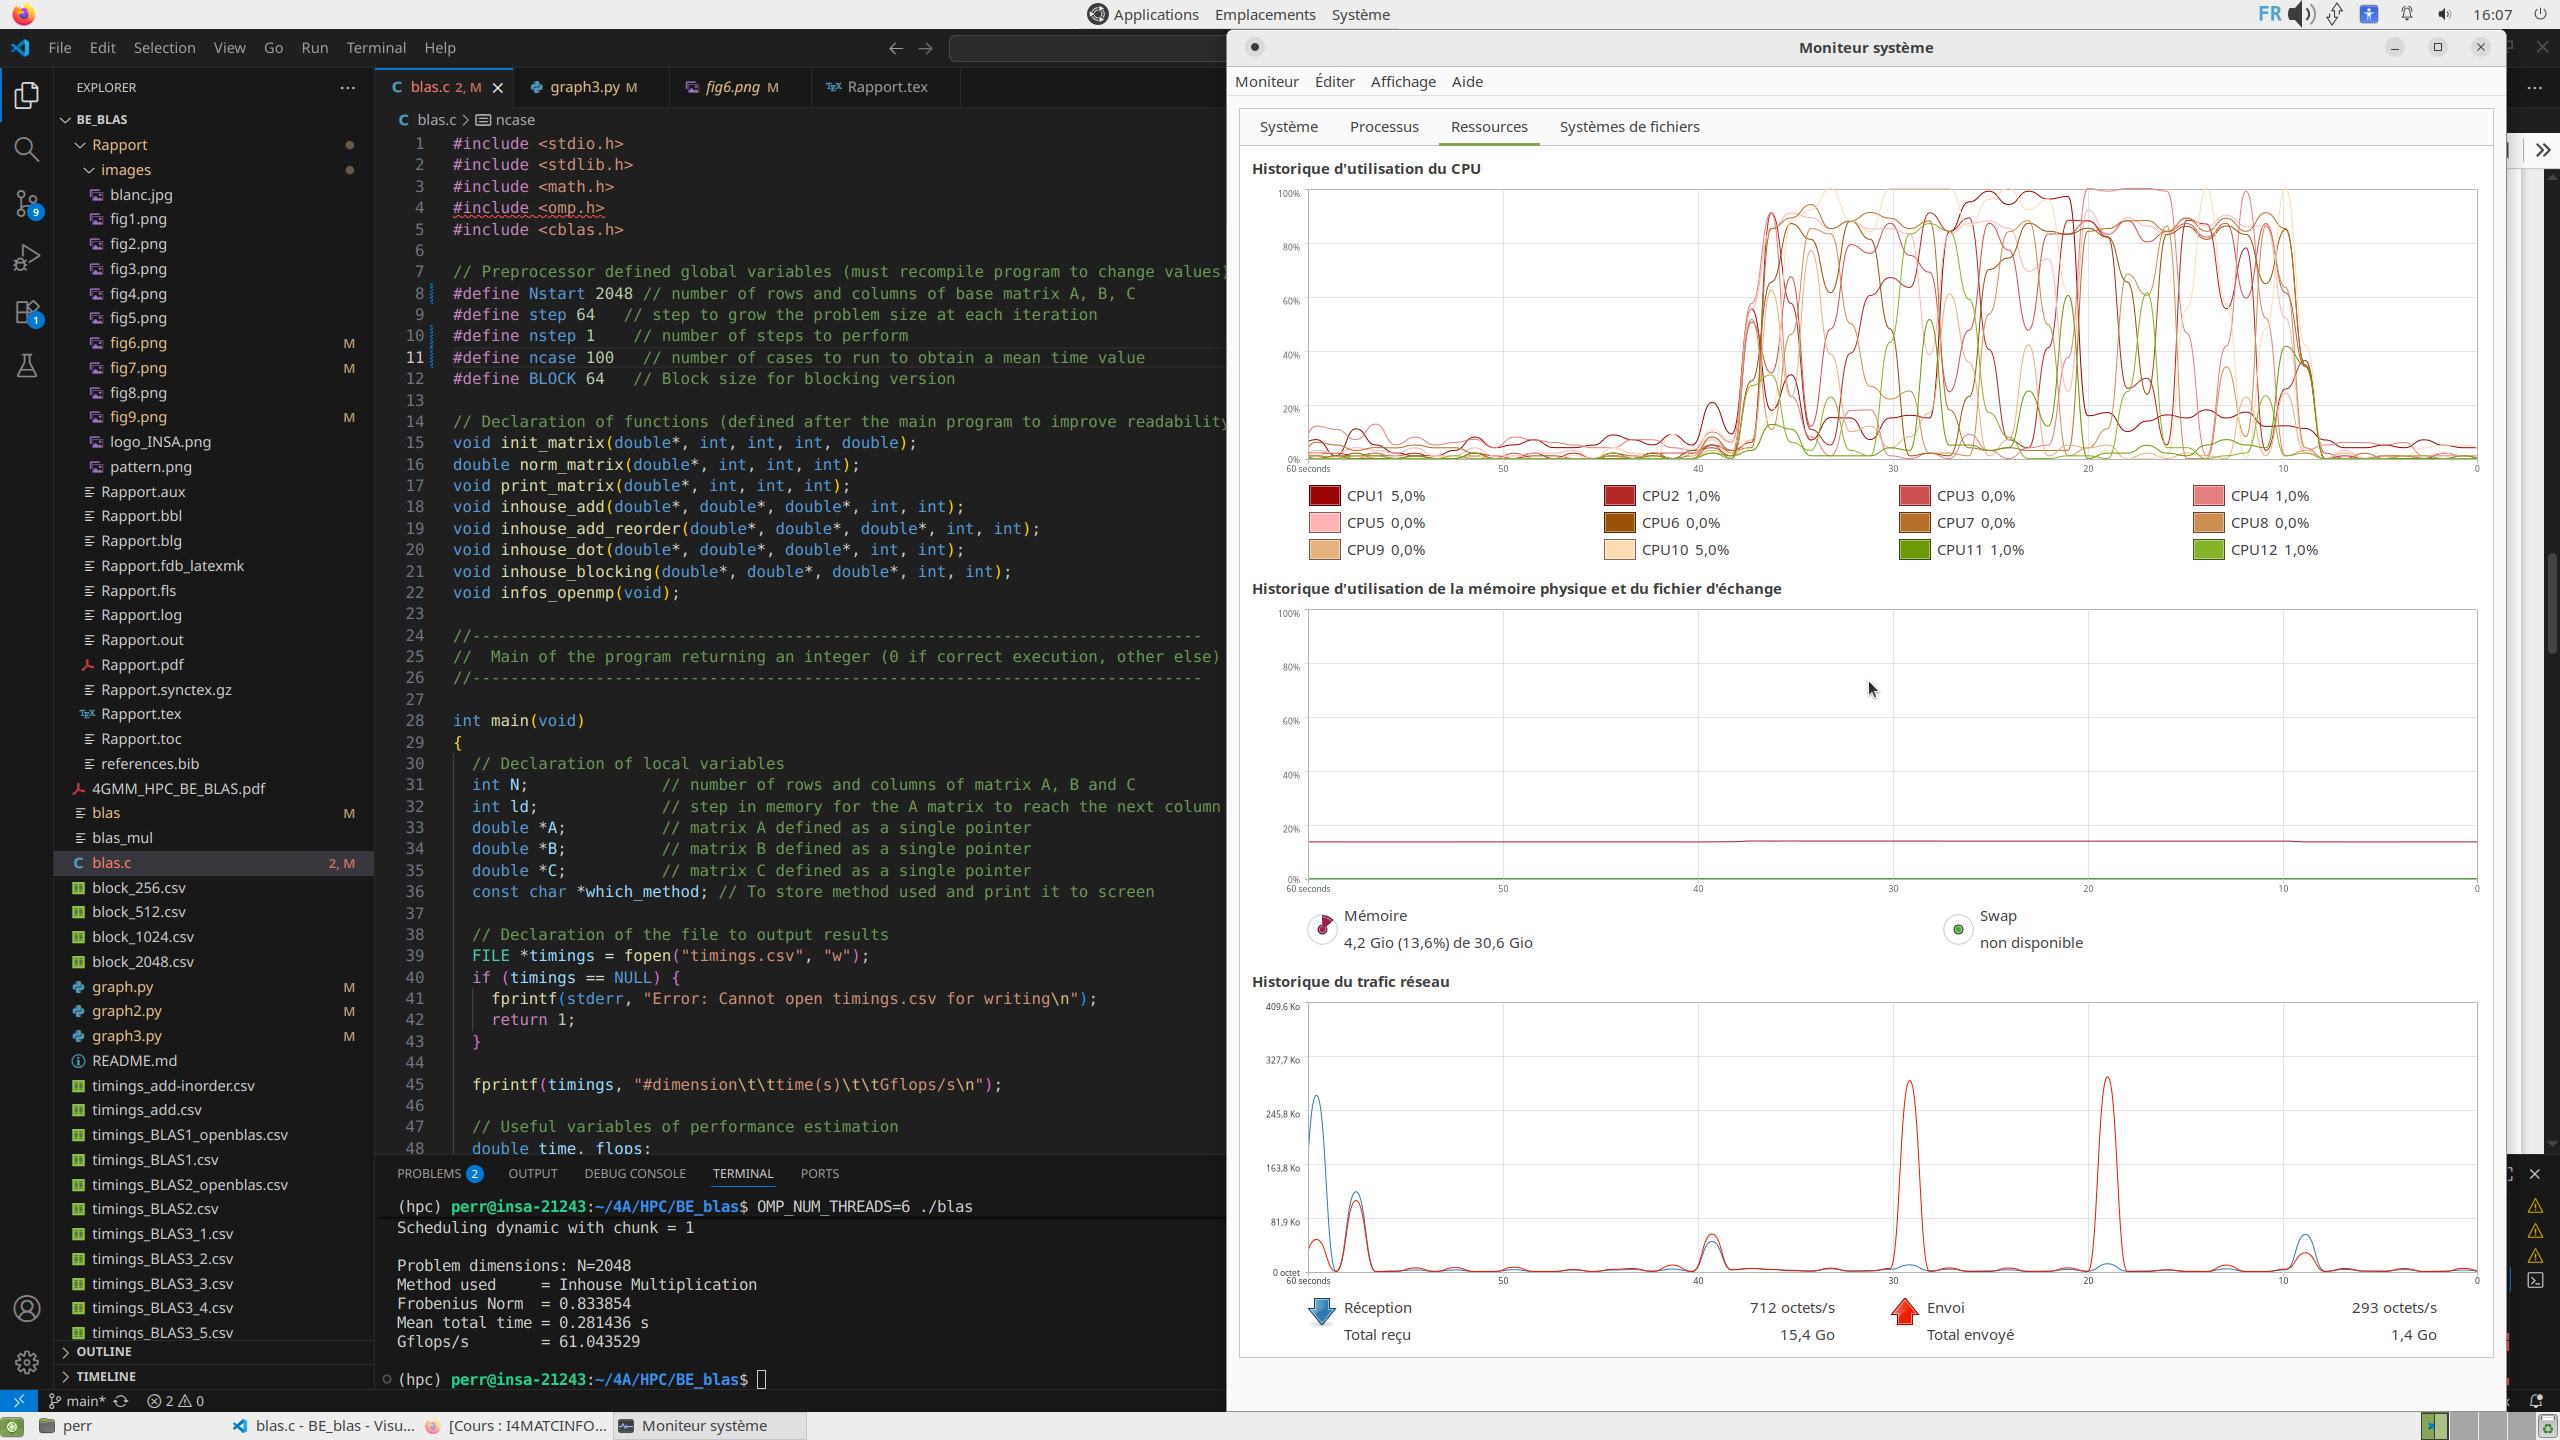
\includegraphics[width=0.7\linewidth]{images/useCPU.png}
    \caption{Trouver titre}
    \label{fig:7}
\end{figure}

Fait des tests de 1 à 12. Le nombre optimal c'est 6 parce que plus on parrallelise, plus on doit partager des données entre les différents threads. 

Expliquer que 6 threads qui ravail en permanence mais ce ne sont pas tout le temps les même.

\chapter{Utiliser les blocs du cache}

Expliquer la technique du block.

\begin{figure}[H]
    \centering
    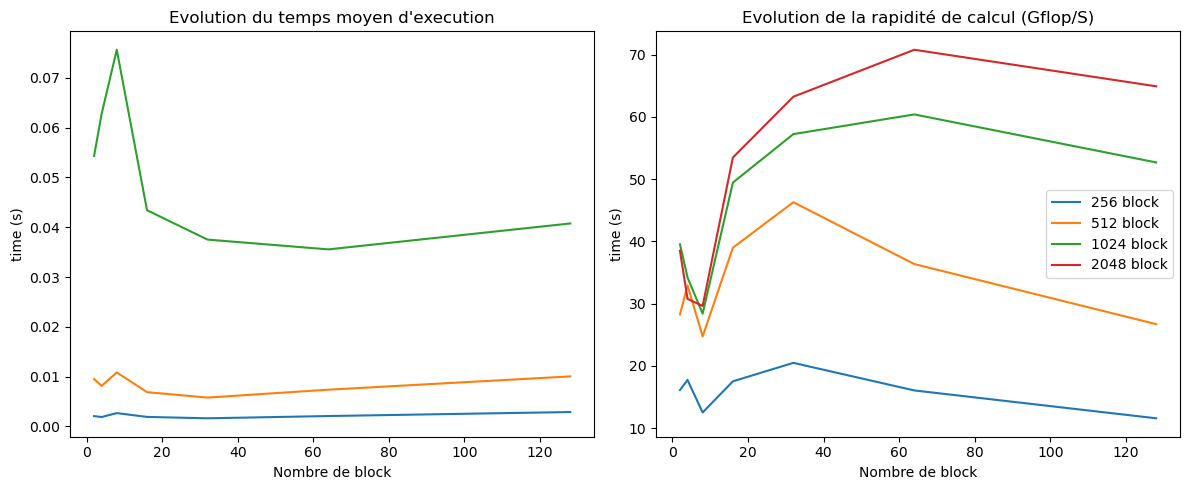
\includegraphics[width=0.7\linewidth]{images/fig7.png}
    \caption{Trouver titre}
    \label{fig:8}
\end{figure}

\begin{figure}[H]
    \centering
    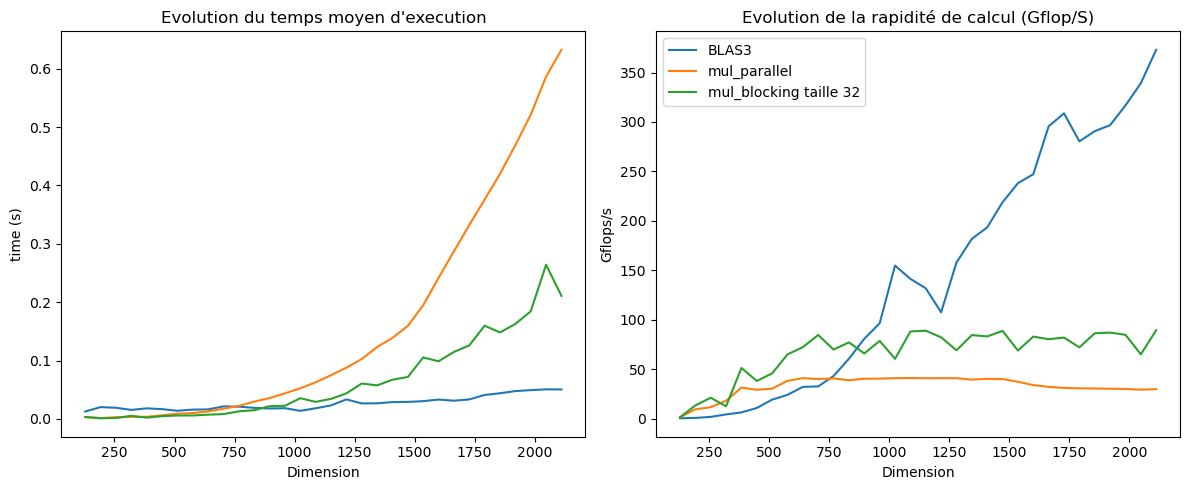
\includegraphics[width=0.7\linewidth]{images/fig9.png}
    \caption{Trouver titre}
    \label{fig:9}
\end{figure}

On a commencé par une rechercher de la taille de block optimale en fonction de différentes tailles de matrices. On a choisi 32 (mieux que 64).

Puis on a comparé cette technique avec openblas et la parralelisation.

On peut observer que la librairie openblas est la meilleure solution pour optimiser les performances de calcul en partageant efficassemet les thread.

\bibliographystyle{plain}
\bibliography{references}


\end{document}